\documentclass[../DS07.tex]{subfiles}
\graphicspath{{./figures/}}

% \subimport{/home/nora/Documents/Enseignement/Prepa/bpep/exercices/DS/oeuf_dur/}{sujet.tex}

\begin{document}

\prblm[32\footnotesize$\times$\num{1.5}]{Rotation d'un œuf
	dur\ifcorrige{~\small\textit{(D'après TPC CCP 2018)}}}

\enonce{
	Le document ci-dessous décrit un phénomène qu'on observe lorsqu'on met en
	rotation un oeuf dur.
	\smallbreak
	\shadowbox{
		\setlength{\fboxsep}{3mm}
		\noindent
		\begin{minipage}{17cm}\textbf{Document A}
			Lorsqu'on impulse un mouvement rotatif très rapide (plus d'une dizaine de
			tours par seconde) à un oeuf dur posé sur une surface bien plane et pas
			trop lisse, il se produit un étrange phénomène. Au bout de quelques tours,
			l'oeuf se dresse et se met à tourner sur sa pointe ou sur sa base~!
			Lorsqu'il perd peu à peu de la vitesse par frottements, il finit par se
			remettre en position couchée, position où son centre de gravité est le
			plus bas.
			\begin{center}
				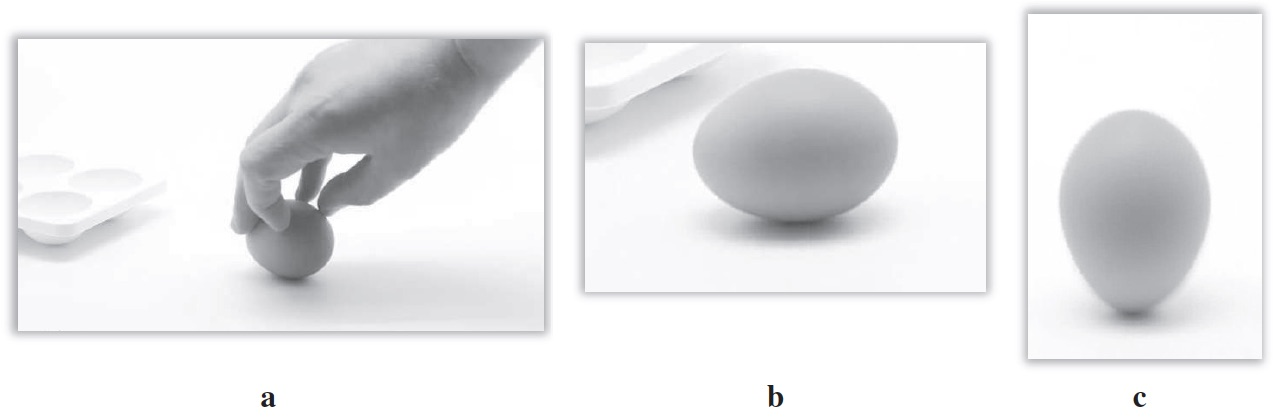
\includegraphics[width=.9\linewidth]{oeuf_2}
			\end{center}
			Évolution d'un oeuf dur en rotation dans l'ordre chronologique a, b et c.
			\begin{flushright}
				\small{\textit{Source~: Le kaléidoscope de la physique, Varlamov,
						Villain, Rigamonti, 2014}}
			\end{flushright}
		\end{minipage}
	}

	\vspace{0.3cm}

	On souhaite établir pour l'oeuf dur la condition de basculement de la position
	horizontale à la position verticale. On adopte le paramétrage de la figure
	\ref{fig:oeuf} ci-dessous~:

	\begin{center}
		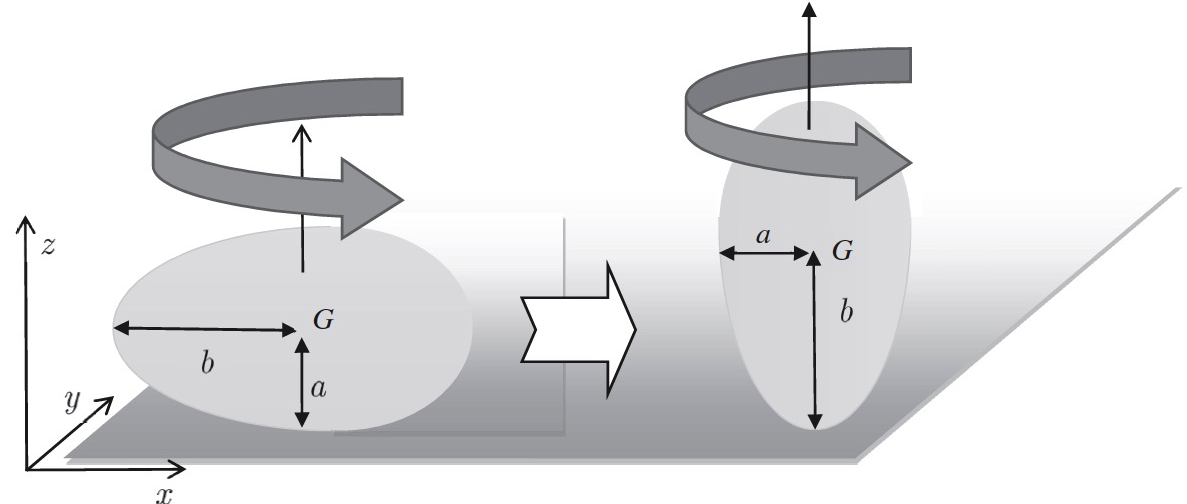
\includegraphics[width=.9\linewidth]{oeuf_1}
		\captionof{figure}{Passage de la position
			horizontale (à gauche) à la position verticale (à droite)}
		\label{fig:oeuf}
	\end{center}

	On ne considère que les états initial et final, on ne s'intéresse pas au
	mécanisme transitoire du redressement de l'oeuf. On modélise l'oeuf dur par un
	ellipsoïde de révolution homogène de masse $m$, de demi petit axe $a$ et de
	demi grand axe $b$ (avec $a<b$). Le centre de masse $G$ est au centre de
	l'ellipsoïde (on néglige la légère asymétrie de l'oeuf). Les moments d'inertie
	d'un ellipsoïde de masse $m$ par rapport à son axe de rotation $Oz$ s'écrivent~:

	\begin{itemize}
		\item $J_H=\frac{1}{5}m(a^2+b^2)$ lorsque l'oeuf tourne à l'horizontal,
		\item $J_V=\frac{2}{5}ma^2$ lorsque l'oeuf tourne à la verticale.
	\end{itemize}
	On pose $\W$ la vitesse de rotation de l'oeuf, qu'il soit dans sa position
	verticale ou horizontale.
}%

%question ajoutée par rapport au sujet
\QR[2]{%
	Comparer les deux moments d'inertie $J_H$ et $J_V$ et commenter physiquement.
}{%
	Comme $b>a$, on a $J_H>J_V$. \pt{1} En effet, la masse est globalement répartie
	plus loin de l'axe de rotation, \pt{1} donc le moment d'inertie est plus grand.
}%

\QR[2]{%
	Exprimer l'énergie mécanique totale de l'oeuf dans les deux positions
	$\Ec_{m_H}$ et $\Ec_{m_V}$ en fonction des données. On choisira comme origine
	de l'énergie potentielle de pesanteur celle d'altitude nulle.
}{%
	Dans les deux cas, $\Ec_m=\Ec_c+\Ec_p=\frac{1}{2}J\W^2+mgz_G$, \pt{1} on a donc
	\[
		\boxed{\Ec_{m_H}=\frac{1}{2}J_H\W^2+mga}
		\stm{\qet}
		\boxed{\Ec_{m_V}=\frac{1}{2}J_V\W^2+mgb}
	\]
}%

\QR[3]{\label{q:pulsLimite}%
	Montrer qu'il existe une pulsation limite $\W_c$ telle que pour $\W>\W_c$, la
	position verticale est d'énergie inférieure à la position horizontale et
	assure le basculement d'une position à l'autre. On donnera l'expression de
	$\W_c$ en fonction de $a$, $b$, et $g$.
}{%
	\label{q:pulsLimite}%
	On cherche la condition sur $\W$ pour avoir $\Ec_{m_V} \stm[-1]{<} \Ec_{m_H}$,
	ce qui équivaut à~:
	\begin{gather*}
		\frac{1}{2}J_V\W^2+mgb <
		\frac{1}{2}J_H\W^2 + mga
		\Lra
		2mg (b-a) <
		(J_H-J_V)\W^2
		\\
		\Lra
		2mg (b-a) \stm{<}
		\frac{m}{5}\underbracket[1pt]{(b^2-a^2)}_{(a-b)(a+b)}\W^2
		\Lra
		\W > \boxed{\W_c \stm{=} \sqrt{\frac{10 g}{a+b}}}
	\end{gather*}
}%

\QR[2]{%
	Calculer $\W_c$ pour $a=\SI{2,0}{cm}$ $b=\SI{3,0}{cm}$ et
	$g=\SI{10}{m.s^{-2}}$. Commenter le résultat obtenu en utilisant les
	descriptions de l'expérience du document.
}{%
	L'application numérique donne $\W_c=\SI{45}{rad.s^{-1}} \pt{1}$, soit environ
	\SI{7}{tour\per\second}. Cette valeur est du bon ordre de grandeur puisqu'on
	nous parle dans le document d'une vitesse de rotation d'une dizaine de tours
	par seconde. \pt{1}
}%

\enonce{
	On suppose que le contact entre l'oeuf et la table se fait sans frottement.
	Dans ce cas, lors du redressement de l'oeuf, l'énergie doit être conservée. On
	fait tourner l'oeuf en position horizontale, avec une vitesse angulaire
	initiale légèrement supérieure à la vitesse limite~:
	$\W_0=\W_c+\ep$ (avec $\ep \ll \W_c$). L'oeuf se
	redresse et tourne alors avec une vitesse angulaire finale $\W_f$ que l'on
	peut écrire sous la forme $\W_f=\W_c+r\ep$ (avec $r$ un nombre
	sans dimension).
}%

\QR[3]{%
	Exprimer les énergies mécaniques initiale $\Ec_{m_H}$ et finale $\Ec_{m_V}$ au
	premier ordre en $\ep$.
}{%
	À l'état initial, on a
	\[
		\Ec_{m_H} =
		\frac{1}{2}J_H\W_0^2 + mga \stm{=}
		\frac{m}{10}(a^2+b^2)(\W_c+\ep)^2 + mga
	\]
	soit au premier ordre en $\ep$ (DL1)~:
	\[
		\boxed{\Ec_{m_H} \stm{=}
			\frac{m}{10}(a^2+b^2)(\W_c^2+2\W_c\ep)+mga}
		\qqet
		\boxed{\Ec_{m_V} \stm{=}
			\frac{m}{5}a^2(\W_c^2+2\W_c\ep r)+mgb}
	\]
}%

\QR[7]{%
	En déduire, d'après les hypothèses, la valeur de $r$ en fonction de $a$ et de
	$b$. L'oeuf a-t-il accéléré ou ralenti lors de son redressement~? Que vaudrait
	$r$ pour $a\approx b$~? Commenter.
}{%
	\leavevmode\vspace*{-15pt}\relax
	\begin{align*}
		\beforetext{$\Ec_{m_H} \stm{=} \Ec_{m_V} \Ra $}
		\frac{m}{5}a^2(\W_c^2+2\W_c\ep r) + mgb & =
		\frac{m}{10}(a^2+b^2)(\W_c^2+2\W_c\ep)+mga
		\tag{1}
		\\\beforetext{Or, \ref{q:pulsLimite} $\Ra$}
		\frac{m}{5}a^2\W_c^2+mgb                & \stm{=} \frac{m}{10}(a^2+b^2)\W_c^2+mga
		\tag{2}
		\\\Ra
		\frac{m}{10}(a^2+b^2)2\W_c\ep           & \stm{=}
		\frac{m}{5}a^22\W_c r\ep
		\tag*{$(3) = (1)-(2)$}
		\\\Lra
		\Aboxed{r                               & \stm{=} \frac{a^2+b^2}{2a^2}}
	\end{align*}
	$b>a$ donc $r>1$ donc $\W_f>\W_0$. \pt{1} Lors de son redressement, la vitesse
	de rotation de l'oeuf augmente.
	\smallbreak
	Dans le cas où $a=b$, c'est-à-dire dans le cas d'un oeuf sphérique, on retrouve
	$r=1$ \pt{1} puisque le système reste inchangé (dans ce cas, on ne peut même plus
	parler de redressement), donc sa vitesse de rotation ne varie pas. \pt{1}
}%

\QR[4]{%
	Exprimer les moments cinétiques $\Lc_H$ et $\Lc_V$ de l'oeuf par rapport à l'axe
	$Oz$ avant et après son redressement. Exprimer la variation de moment
	cinétique $\Delta \Lc=\Lc_V-\Lc_H$ en fonction de $\W_c$, $m$, $a$ et $b$.
	L'oeuf a-t-il gagné ou perdu du moment cinétique lors de son redressement~?
}{%
	\leavevmode\vspace*{-15pt}\relax
	\begin{gather*}
		\boxed{\Lc_H = J_H\W_0=\frac{m}{5}(a^2+b^2)(\W_c+\ep)}
		\stm{\qet}
		\boxed{\Lc_V = J_V\W_f=\frac{2m}{5}a^2(\W_c+r\ep)}
		\\\Ra
		\Delta \Lc \stm{=} \frac{m}{5}(a^2-b^2)\W_c+\frac{m}{5}(2a^2r-a^2-b^2)\ep
		\\\beforetext{$r = \frac{a^2+b^2}{2a^2} \Ra$}
		\boxed{\Delta \Lc \stm{=} \dfrac{m}{5}(a^2-b^2)\W_c < 0}
	\end{gather*}
	\smallbreak
	Le moment cinétique de l'oeuf a diminué lors de son redressement. \pt{1}
}%

\QR[5]{%
	Cette variation de moment cinétique signifie que, pendant le temps $\Delta t$
	du redressement, l'oeuf a subi un couple $\Gf$. Montrer que la composante
	verticale de ce couple par rapport à l'axe $Oz$ peut s'écrire~:
	\[
		\G_z\approx \dfrac{2mg(a-b)}{\W_c\Delta t}
	\]
	Commenter son signe.
}{%
	D'après le théorème du moment cinétique, on peut écrire $\dv{\Lc}{t} = \G_z$.
	\pt{1} En supposant que le redressement est de courte durée, on peut approcher
	$\dv{\Lc}{t}$ par $\frac{\Delta \Lc}{\Delta t}$, on a donc
	\[
		\G_z =
		\frac{m}{5}(a^2-b-2)\frac{\W_c}{\Delta t} \stm{=}
		\frac{m}{5}(a^2-b-2)\frac{\W_c^2}{\W_c\Delta t}
	\]
	On injecte l'expression de $\W_c$ obtenue à la question~\ref{q:pulsLimite}~:
	\[
		\boxed{
			\G_z =
			\frac{m}{5}(a^2-b^2)
			\frac{10 g}{(a+b)\W_c\Delta t} \stm{=}
			\frac{2mg(a-b)}{\W_c\Delta t}}
	\]
	Ce couple est négatif, \pt{1} ce qui est cohérent avec le fait que le moment
	cinétique de l'oeuf ait diminué pendant le redressement. \pt{1}
}%

\QR[4]{%
	Le poids ou la réaction normale du support peuvent-ils être responsables d'un
	tel couple~? Si non, d'où peut provenir ce couple~? Y a-t-il une contradiction
	avec les hypothèses de l'énoncé~?
}{%
	Le poids et la réaction normale ne peuvent \pt{1} pas être responsable d'un
	tel couple car ces deux forces sont parallèles à l'axe de rotation, donc leur
	moment par rapport à cet axe est nul \pt{1}. Ce couple peut éventuellement
	provenir des frottements, \pt{1} car on nous dit dans le document qu'il faut
	que la surface ne soit «~pas trop lisse~». Cependant, cela contredit
	l'hypothèse de l'énergie mécanique constante. \pt{1}
}%

\end{document}
